\section{Introduction}

\label{sec:Intro}
Graph privacy issues are becoming increasingly important for many applications such as business to business, social networks and instant-messaging networks. 
This is evidenced by the fact the responsible management of sensitive personal information is explicitly mandated through regulations such as European Union's General Data Protection Regulation.
% There are public concerns on how data companies collect personal information and make it available to marketers. 
Users are afraid that the sensitive personal information can be exploited in harmful ways (e.g., cyberstalking).
Meanwhile, data companies have strong fears of violating privacy regulations. 
Accordingly, there has 
been considerable interest in publishing graph data or analysis result under certain privacy guarantees~\cite{Liu_Towards_2008,Wang2011,Liu_Privacy_2009,Nguyen_Anonymizing_2015,Sala_Sharing_2011,Xiao_Differentially_2014,lee2011}. 
However, the majority of works has been limited to the deterministic scenario. 

In some applications, the graph may be probabilistic by nature. 
For example, in social networks, an edge between two individuals corresponds to an interaction or the influence that is predicted through machine learning models characterized by some level of uncertainty, which can thus be conveniently presented as the probability of the existence of that edge~\cite{Adar_Managing_2007,Kempe_Maximizing_2003}. In these situations, the problem of privacy protection becomes far challenging. 

\textbf{Uncertainty: critical privacy factors}~~First, edge uncertainty contains sensitive information about individuals such as a user's influence in a community or over another individual. 
For example, if we consider a small community, the members and the link structures of the members are known to any participant who is also a member of the community. However, the edge uncertainty such as the ``trustworthiness" of user A to user B should be private.
Second, the extra release of edge uncertainty makes the user identity more vulnerable. 
For example, if we consider a small community, several ``trustworthiness" connections between members are known to an intruder who is also a member of the community. The intruder can match the released probabilistic graph with known information, and serves in privacy attacks.  

\textbf{Uncertainty: critical utility factors} Meanwhile, these probabilistic graph are valuable for research and applications such as marketing and advertising, friend recommendation and modeling the structure and dynamic where uncertainty plays a indispensable role. For example, effective advertising needs to leverage the trust and influence relationships among users (uncertainty) as they may greatly impact users' behavior, as illustrated in Figure~\ref{fig:motivationExample}.  The primitive of these applications is to categorize and compute reachability between any two nodes. Therefore, it is these properties of edge uncertainty that must be preserved. 

\textbf{The limitation of existing methods}~~
In these situation, existing solutions for privacy protection graph publication and analysis do not apply because of the ignorance of edge uncertainty. 

Together, it calls for fundamental anonymization primitives for publishing uncertain graphs which, as ever-argued, would become different from the deterministic ones.

\textbf{Challenge} 
The challenges in privacy-preserving uncertain graph publishing are both semantics and computation driven. 

\textbf{What to xxxx}
% From the perspective of the semantics, there is no privacy notation and utility loss metrics over the probabilistic scenario.   First, it is much more challenging to model attacks where the background knowledge and released data both are probabilistic. 
% Second, it is much more challenging to model the utility loss over 


\textbf{How to anonymize uncertain graph efficiently ?}~~While many graph anonymization algorithms such as k-automorphism are intrinsically hard problems, even the simplest degree anonymization by  contractions with minimal loss of information is known to be NP-hard in the deterministic cases~\cite{}. In the probabilistic scenario, edge modifications are no longer limited to edge addition and deletions but can be infinite probability deviation,hence, more expensive over uncertain graphs. Therefore, exact computation is infeasible with today's large-scale graph data. 
Meanwhile, approximation methods designed for deterministic graphs does not guarantee efficiency and in uncertain graphs. For example, xx xx  

\textbf{Our contribution} In this paper we develop novel strategies for sanitizing uncertain graph with dynamic sampling, and filtering strategies. 
One key idea is that Squid captures the structure
of the original decentralized graph, by incrementally identifying
and refining clusters of connected nodes under local differential
privacy. 
To do so, Squid iteratively xxx.
After obtaining such node clusters, it applies a graph
generation model that utilizes such groups to generate a representative
synthetic social graph. Also, we describe techniques to
optimize critical parameters of xxx to improve the utility of the
generated synthetic social graph.


To validate the effectiveness of Squid, we present an extensive
set of experiments using three real uncertain graphs in various
domains, and two different use cases: (i) statistical analysis of the
 graph structure, (ii) influence propagation. 
 
The experiment results show that synthetic
 generated using Squid obtains high utility for all
use cases and datasets, whereas baseline solutions fail to capture
competitive utility in most settings except for the few that they are
specifically optimized for. 

Our main contributions are summarized as follows: 
\begin{itemize}
\item We formulate the problem of synthetic data generation of uncertain graph under syntactic anonymity while keeping the data utility in mind. To this end, we propose a reliability-driven utility loss metric, which evaluates the connectivity difference in the context of the entire graph and also utilizes the possible world model.  

\item We propose Squid, a novel and effective randomized algorithm to synthetic uncertain graph generation and describe methods for scaling computation. Boosted by the hybrid of uncertainty-aware heuristics, it excels in identifying a population of synthetic results with good quality efficiently. 

\item We conduct a comprehensive experimental study using several
real datasets and use cases. The results demonstrate that
Squid improves the utility of
obtained result, while providing users with their desired privacy guarantees. 
\end{itemize}

\begin{figure}
    \centering
    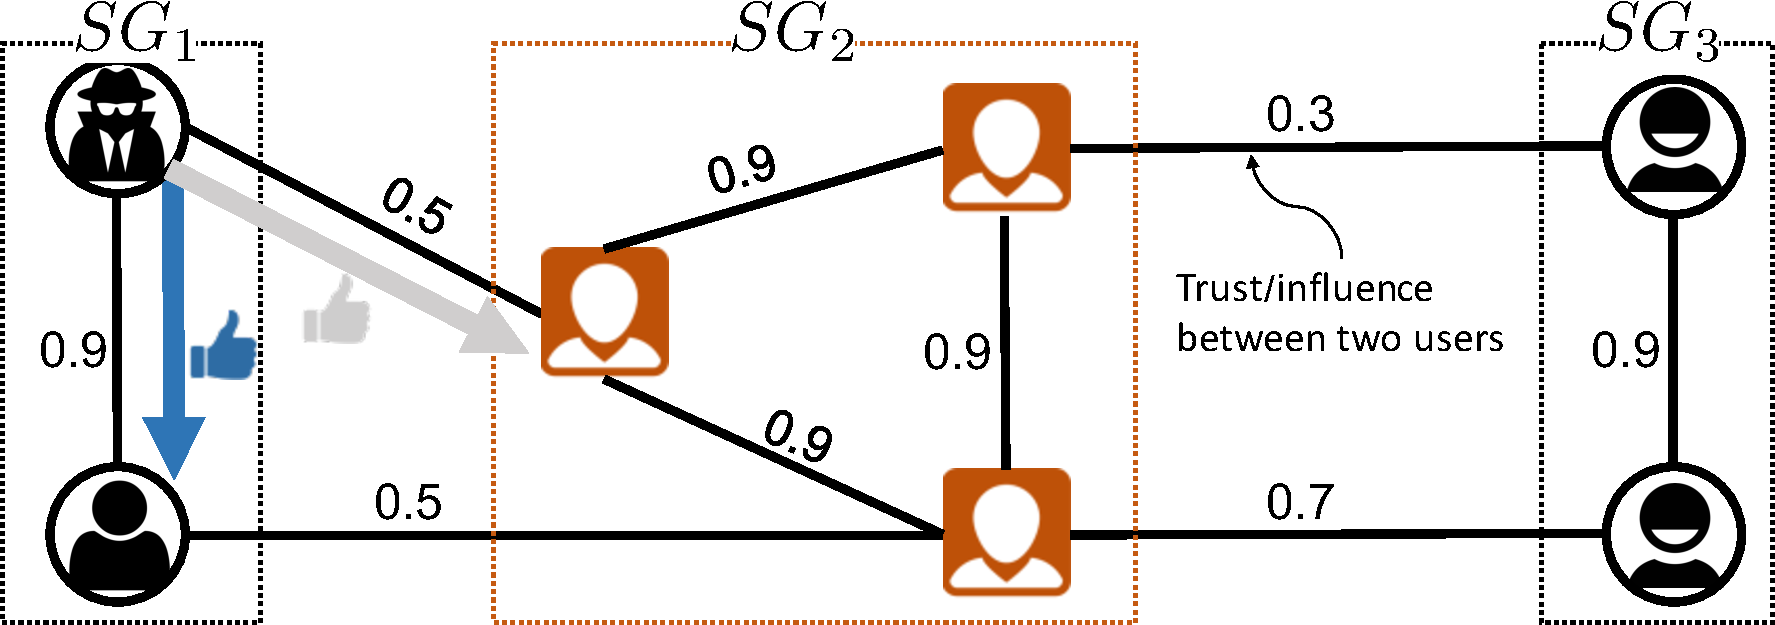
\includegraphics[height=2.3cm] {figure/motivationExampleWideWithApplication.pdf}
    \caption{ An Motivation Example}
    \vspace{-10pt}
    \label{fig:motivationExample}
\end{figure}

% \begin{figure}[t]
%     \subfigure[Social Trust Network]{\label{fig:socialNetwork}
%       \begin{minipage}[l]{0.40\columnwidth}
%         \centering
%         \includegraphics[height=2.3cm]{ill/SocialNetwork.pdf}
%       \end{minipage}
%       }
%     \subfigure[B2B Network]{\label{fig:b2bNetwork}
%       \begin{minipage}[l]{0.40\columnwidth}
%         \centering
%         \includegraphics[height=2.3cm]{ill/B2BNetwork.pdf}
%       \end{minipage}
%       }
%     \vspace{-6pt}
%     \caption{Real uncertain graphs with privacy concerns.}
%     \vspace{-10pt}
%     \label{fig:motivation}
% \end{figure} 


The rest of the paper is organized as follows. In Section~\ref{sec:relatedWork}, we summarize related works, point out the limitation of existing methods, and clarify our distinct privacy goal. In Section~\ref{sec:notation} we formulate the uncertain graph-anonymization problem. Sections~\ref{sec:soa}--\ref{sec:method} present our anonymization approach for privacy-preserving uncertain graph sharing.  In Section~\ref{sec:ex} we apply our method to several real-world uncertain graphs and demonstrate its performance, practical utility, and efficiency. 